% !TEX program = xelatex

\documentclass[aspectratio=169]{beamer}

\usepackage{xltxtra} 
\usepackage{fontspec}
\usepackage{listings}
\usepackage{color}
\usepackage{amsmath}
\usepackage{smartdiagram}
\usepackage{graphicx}
\usepackage{multicol}
\usepackage{tikz}
\usepackage{listings}
\usepackage{multicol}


\usetheme{metropolis}
\XeTeXlinebreaklocale "th_TH"
\defaultfontfeatures{Mapping=tex-text,Scale=MatchLowercase}

\definecolor{codegreen}{rgb}{0,0.6,0}
\definecolor{codegray}{rgb}{0.5,0.5,0.5}
\definecolor{codepurple}{rgb}{0.58,0,0.82}
\definecolor{backcolour}{rgb}{0.95,0.95,0.92}

\definecolor{terminalbg}{HTML}{1D1F21}
\definecolor{terminalfg}{HTML}{C5C8C6}

\lstdefinestyle{defaultstyle}{
    backgroundcolor=\color{backcolour},   
    commentstyle=\color{codegreen},
    keywordstyle=\color{magenta},
    numberstyle=\tiny\color{codegray},
    stringstyle=\color{codepurple},
    basicstyle=\ttfamily,
    breakatwhitespace=false,         
    breaklines=true,                 
    captionpos=b,                    
    keepspaces=true,                 
    numbers=left,                    
    numbersep=5pt,                  
    showspaces=false,                
    showstringspaces=false,
    showtabs=false,                  
    showlines=false,
    tabsize=4,
    language=python
}

\lstdefinestyle{terminal}{
    backgroundcolor=\color{terminalbg},   
    basicstyle=\ttfamily\color{terminalfg},
    breakatwhitespace=false,         
    breaklines=true,                 
    captionpos=b,                    
    keepspaces=true,                 
    showspaces=false,                
    showstringspaces=false,
    showtabs=false,                  
    showlines=false,
    tabsize=4
}

\lstset{
	escapeinside=||
}

\title{Python for Data Science}
\author{Sirakorn Lamyai}
\institute{Student, Kasetsart U.}

\begin{document}

\maketitle

\begin{frame}
    \frametitle{About me}
    \begin{columns}
        \column{0.3\textwidth}
            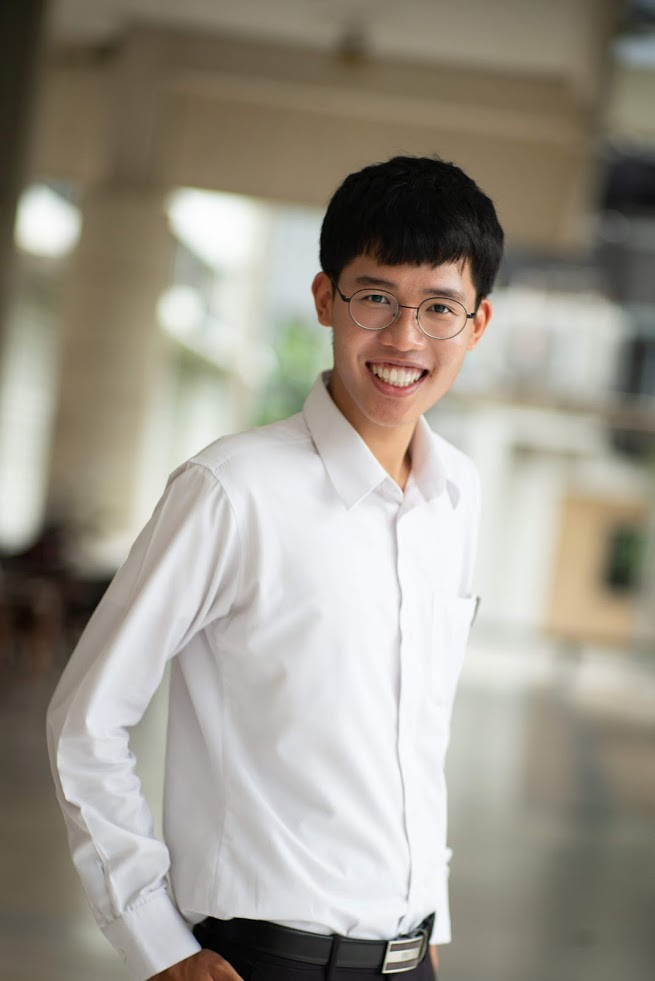
\includegraphics[height=0.8\textheight]{images/sirakorn-1.jpeg}
        \column{0.7\textwidth}
            {\large \textbf{Sirakorn Lamyai}}
            \begin{itemize}
                \item DAKDL Laboratory, Kasetsart University
                \item Research Assistant Intern, 2019, Vidyasirimedhi Institute of Science and Technology
                \item Research Assistant Intern, 2018, Vidyasirimedhi Institute of Science and Technology
                \item Love drinking tea
                \item Knows a little about Python
            \end{itemize}
    \end{columns}
\end{frame}

\begin{frame}
    \frametitle{I know a little about Python}
    When I say I know \textit{a little} about Python\dots
    \begin{itemize}
        \item I think there's some better methods than I'm using
        \item I think I do sometimes make mistakes
        \item There are tons of people who know things much more than me
        \item I think there's much more for me to learn!
    \end{itemize}
\end{frame}

\begin{frame}
    \frametitle{Prerequisite}
    A basic Python knowledge will do!
\end{frame}

\begin{frame}
    \frametitle{Your expectations from this talk}
\end{frame}

\begin{frame}
	\frametitle{Outline}
    \tableofcontents
\end{frame}

\section{Data Science}

\begin{frame}
    \frametitle{The Data Science Process: OSEMNI}
    \begin{itemize}
        \item \textbf{Obtain} data from relevent sources
        \item \textbf{Scrub}, sanitise, and clean the data into machine-understandable formats
        \item \textbf{Explore} significant and meaningful patterns with statistical methods
        \item \textbf{Model} construction for prediction and forecast
        \item \textbf{iNterpret} and use the results obtained
        \item \textbf{Interate} and rethink about your outputs
    \end{itemize}
\end{frame}

\begin{frame}
    \frametitle{Why data?}
    \centering
    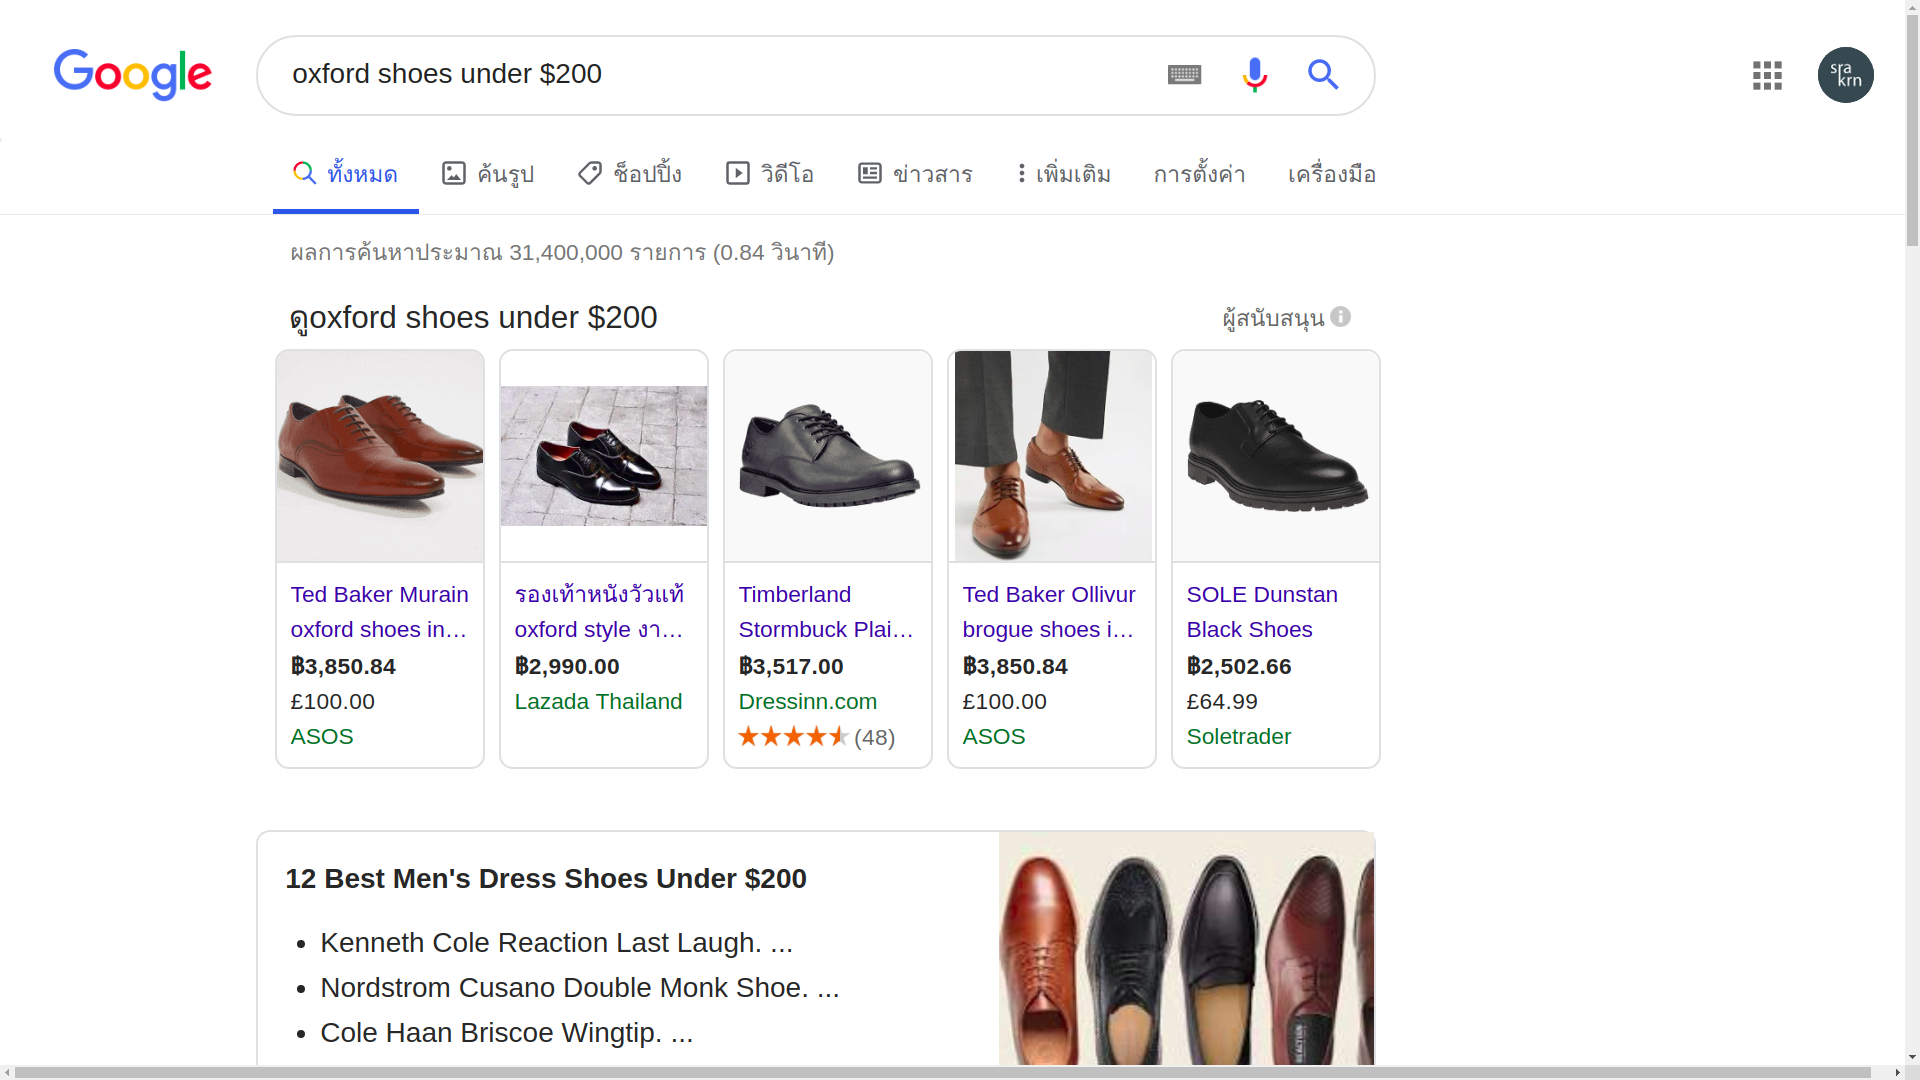
\includegraphics[width=0.8\textwidth]{images/leather-shoes-google.png}
\end{frame}

\begin{frame}
    \frametitle{Why data?}
    \centering
    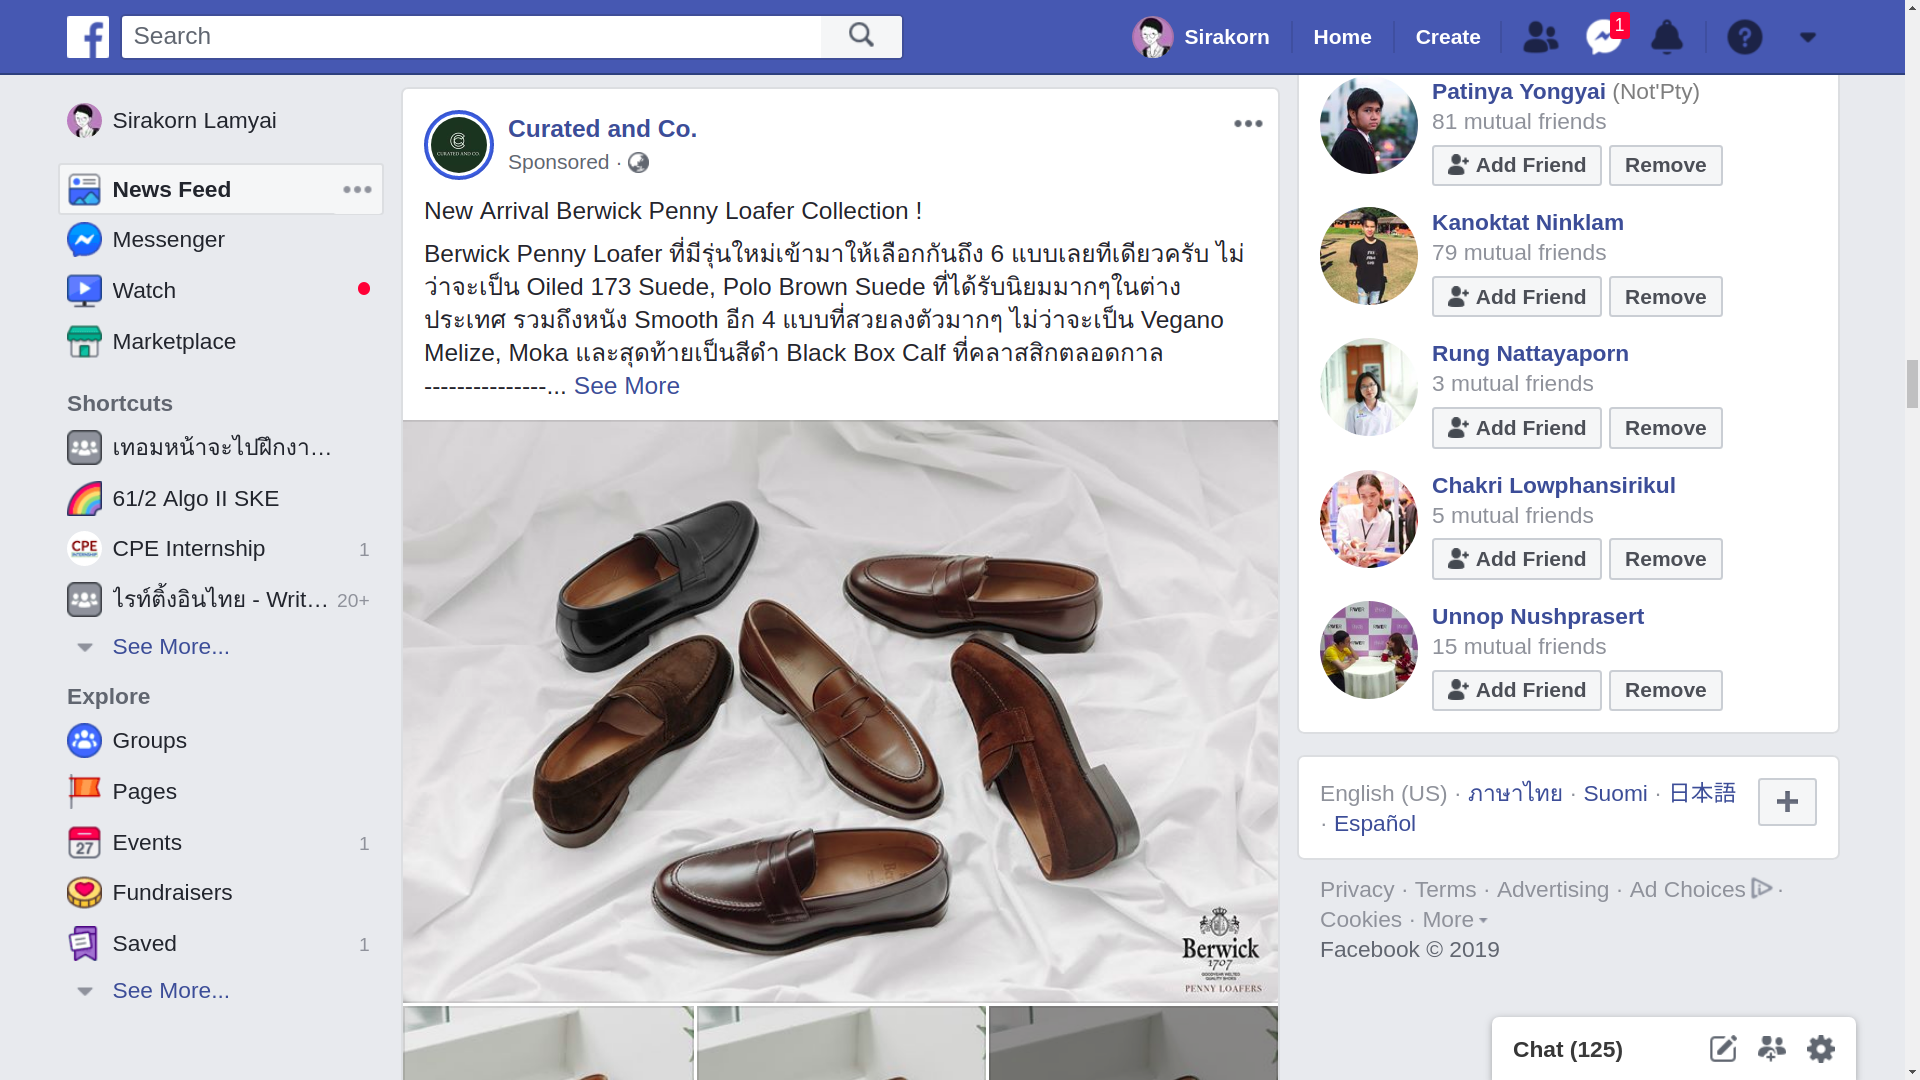
\includegraphics[width=0.8\textwidth]{images/facebook-ads.png}
\end{frame}

\begin{frame}
    \frametitle{Why data?}
    \centering
    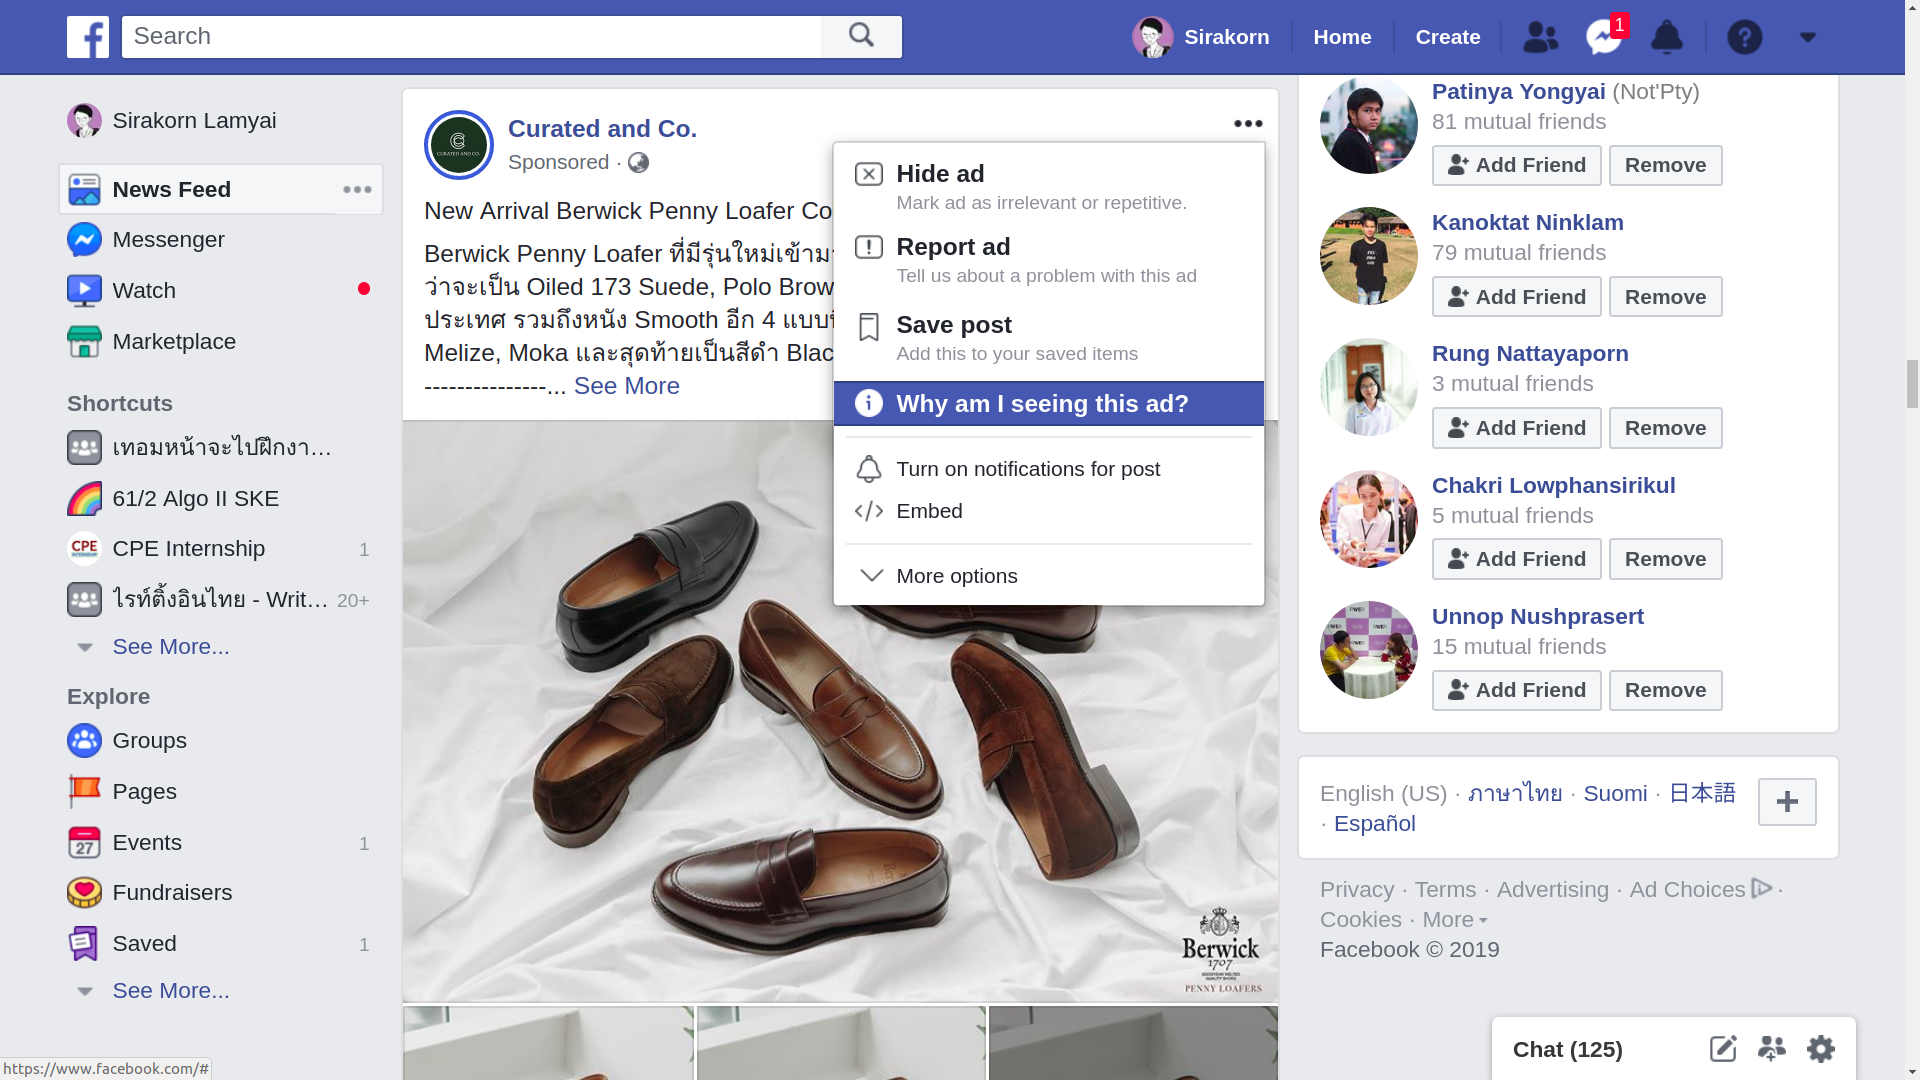
\includegraphics[width=0.8\textwidth]{images/facebook-ads-why-am-i-seeing.png}
\end{frame}

\begin{frame}
    \frametitle{Why data?}
    \centering
    % Zoom 175% on Chrome on Linux to replicate screenshot at this scale
    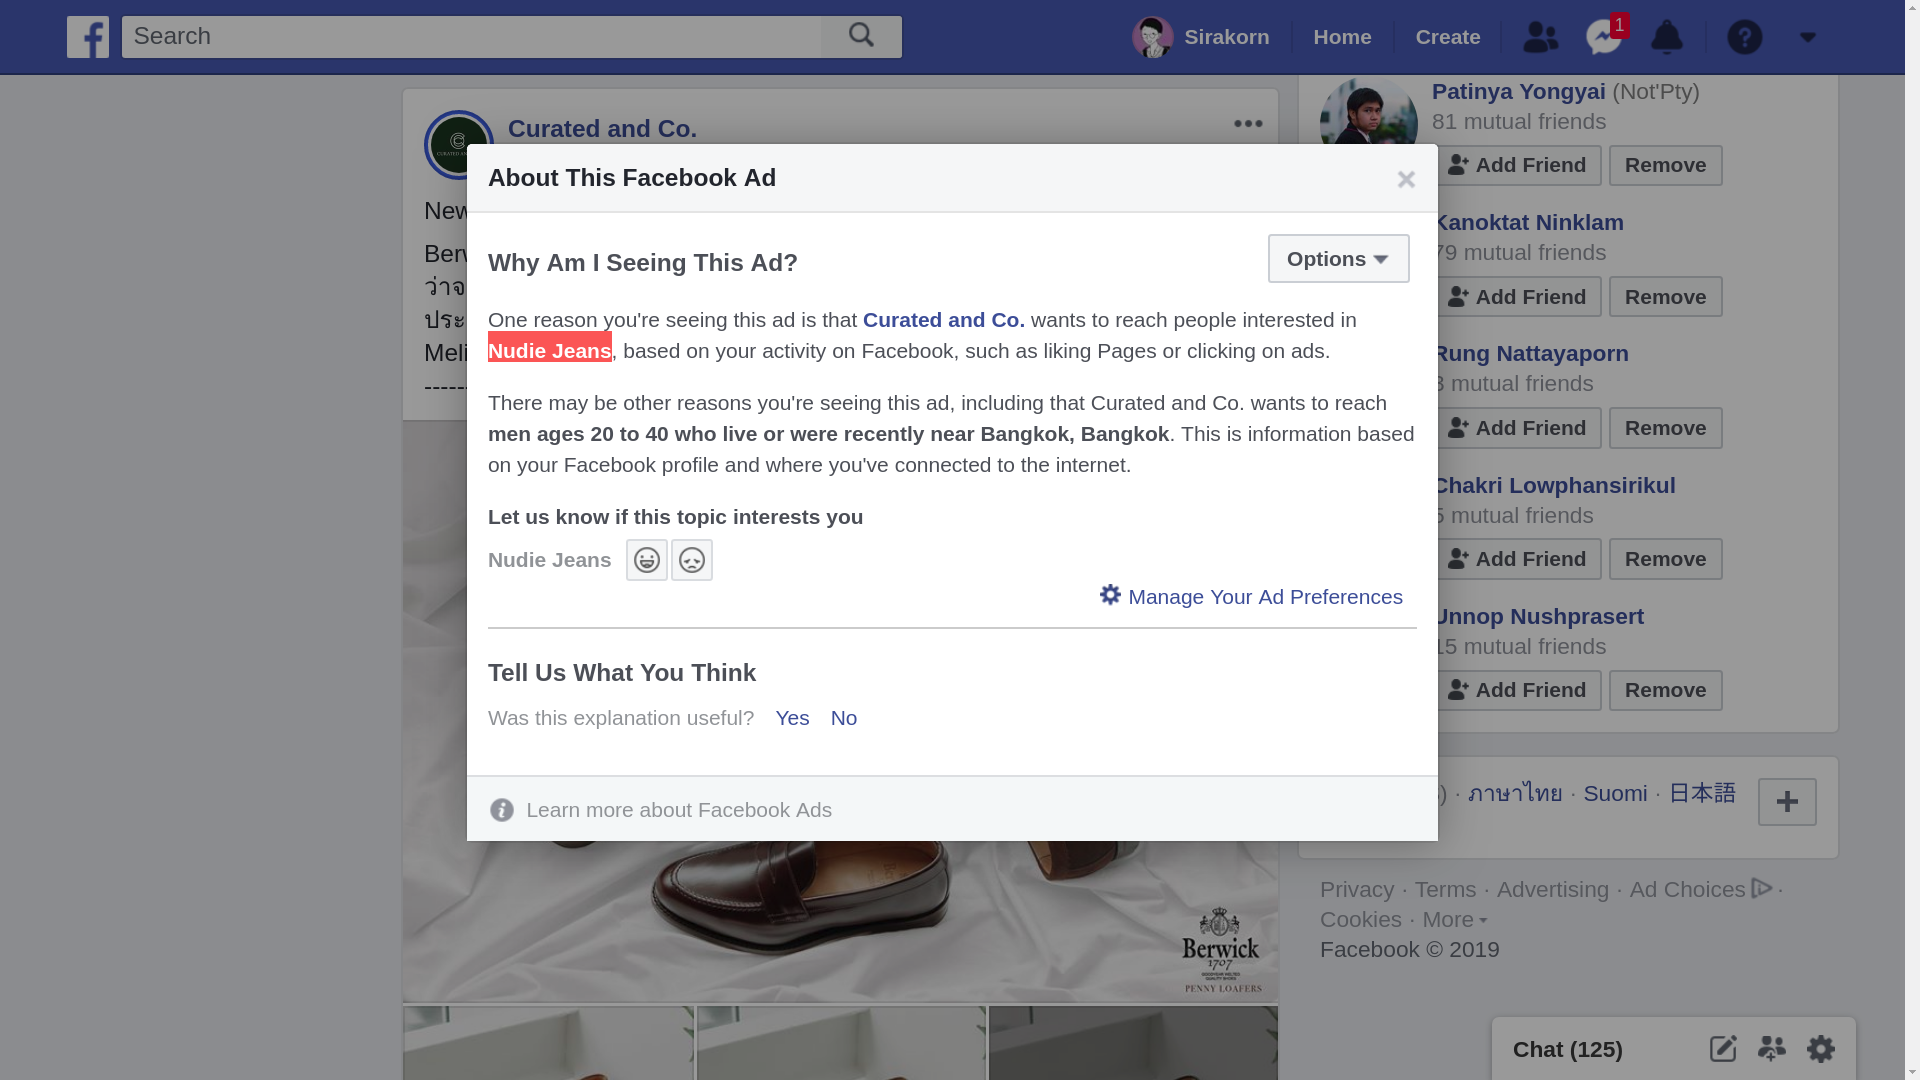
\includegraphics[width=0.8\textwidth]{images/facebook-ads-details.png}
\end{frame}

\begin{frame}
    \frametitle{Why data?}
    \centering
    \Huge Data is the new oil
\end{frame}

\begin{frame}
    \frametitle{Tools for data analysis}
    \begin{columns}[t]
        \column{0.5\textwidth}
            {\large \textbf{With GUIs}}
            \begin{itemize}
                \item Spreadsheets
                \begin{itemize}
                    \item Excel
                    \item Google Spreadsheets
                    \item Lotus 1-2-3
                \end{itemize}
                \item Modelling and Visualisation
                \begin{itemize}
                    \item RapidMiner Studio
                    \item Weka
                    \item Tableau
                \end{itemize}
            \end{itemize}
        \column{0.5\textwidth}
            {\large \textbf{As programming languages}}
            \begin{itemize}
                \item For data insights
                \begin{itemize}
                    \item R
                    \item Python
                \end{itemize}
                \item For data retrieval
                \begin{itemize}
                    \item SQL
                \end{itemize}
            \end{itemize}
    \end{columns}
\end{frame}

\section{Python}

\begin{frame}
    \frametitle{Python}
    \centering
    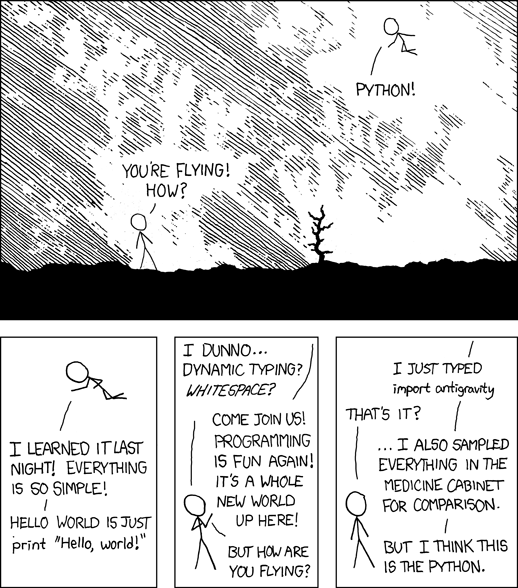
\includegraphics[scale=0.3]{images/xkcd-python.png}

    {\small Courtesy: xkcd (\url{https://xkcd.com/353/})}
\end{frame}

\begin{frame}
    \frametitle{I \textit{loved} Python...}
    \begin{itemize}
        \item Read it, understand it
        \item Multiparadigm
        \item Batteris included
        \item Lots of great, great libraries!
    \end{itemize}
\end{frame}

\begin{frame}
    \frametitle{Python Packages}
    \begin{columns}
        \column{0.4\textwidth}
            \begin{center}
                {\onslide<2-> \Huge \texttt{pip}}
            \end{center}
        \column{0.6\textwidth}
            \begin{itemize}[<+(2)->]
                \item \textbf{PyPA} (\textbf{Py}thon \textbf{P}ackaging \textbf{A}uthority)'s recommended package installer
                \item Obtains packages from \textbf{PyPI} (\textbf{Py}thon \textbf{P}ackaging \textbf{I}ndex)
                \item Many useful packages for us to use!
            \end{itemize}
    \end{columns}
\end{frame}

\begin{frame}
    \frametitle{Anaconda Python Distribution}
    \begin{columns}
        \column{0.4\textwidth}
            \begin{center}
                \includegraphics<2->[width=0.8\columnwidth]{images/anaconda_logo.png}
            \end{center}
        \column{0.6\textwidth}
            \begin{itemize}[<+(2)->]
                \item Cross-platform Python Distribution
                \item Ships with its own package and environment manager
                \begin{itemize}
                    \item Its environment manager capability is not found in Python vanilla installation
                    \item Fetches the packages from its own repository, not PyPI
                \end{itemize}
                \item Aims for Data Science use
                \item \textbf{Entirely separated Python}
            \end{itemize}
    \end{columns}
\end{frame}

\subsection{Python environments}

\begin{frame}[fragile]
    \frametitle{Environments 101: \texttt{\$PATH}}
    \begin{lstlisting}[style=terminal]
$ echo $PATH
/home/srakrn/.pyenv/plugins/pyenv-virtualenv/shims:/home/srakrn/.pyenv/shims:/home/srakrn/.pyenv/bin:/home/srakrn/.local/bin:/usr/local/bin:/usr/local/sbin:/home/srakrn/.local/bin:/usr/sbin:/usr/bin:/sbin:/bin:/usr/games:/usr/local/games:/snap/bin\end{lstlisting}
\end{frame}

\begin{frame}[fragile]
    \frametitle{Different machines, different Pythons}
    On my laptop...
    \begin{lstlisting}[style=terminal]
srakrn@epsilon-ubuntu:~$ which python
/home/srakrn/.pyenv/shims/python\end{lstlisting}
    On my \href{charles}{https://charles.srakrn.me/} server...
    \begin{lstlisting}[style=terminal]
srakrn@charles:~$ which python
/usr/bin/python
srakrn@charles:~$ which python3
/usr/bin/python3\end{lstlisting}
\end{frame}

\begin{frame}[fragile]
    \frametitle{Installed pip}
    \begin{lstlisting}[style=terminal]
$ pip -V 
pip 8.1.1 from /usr/lib/python2.7/dist-packages (python 2.7)
$ pip3 -V 
pip 8.1.1 from /usr/lib/python2.7/dist-packages (python 3.6)\end{lstlisting}
\end{frame}

\begin{frame}
    \frametitle{Perhaps now you understand me...}
    \centering
    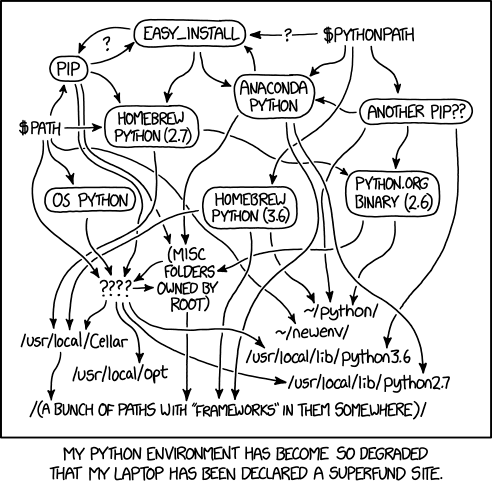
\includegraphics[scale=0.35]{images/xkcd-python-env.png}

    {\small Courtesy: xkcd (\url{https://xkcd.com/1987/})}
\end{frame}

\subsection{Jupyter}

\begin{frame}
    \frametitle{Jupyter}
    \begin{columns}
        \column{0.4\textwidth}
        \begin{center}
            \includegraphics<2->[width=0.7\columnwidth]{images/jupyter-logo.pdf}
        \end{center}
        \column{0.6\textwidth}
        {\onslide<3-> {\LARGE Interactive computing environment}}
    \end{columns}
\end{frame}

\begin{frame}
    \frametitle{Jupyter Notebook}
\end{frame}

\begin{frame}
    \frametitle{Google Colaboratory (Colab)}
    \begin{columns}
        \column{0.4\textwidth}
            \begin{center}
                \includegraphics<2->[width=\columnwidth]{images/colab-logo.png}
            \end{center}
        \column{0.6\textwidth}
        \begin{itemize}[<+(2)->]
            \item Think of an online Jupyter Notebook provided by Google
            \item The runtime relies on Google's server fram
            \begin{itemize}
                \item In other words, your code are remotely executed
            \end{itemize}
            \item Could be more powerful for some tasks (like Deep Learning) than your computer
            \item Free!
        \end{itemize}
    \end{columns}
\end{frame}

\begin{frame}
    \frametitle{Google Colaboratory (Colab)}
    \centering
    \huge \url{https://colab.research.google.com/}
\end{frame}

\begin{frame}
    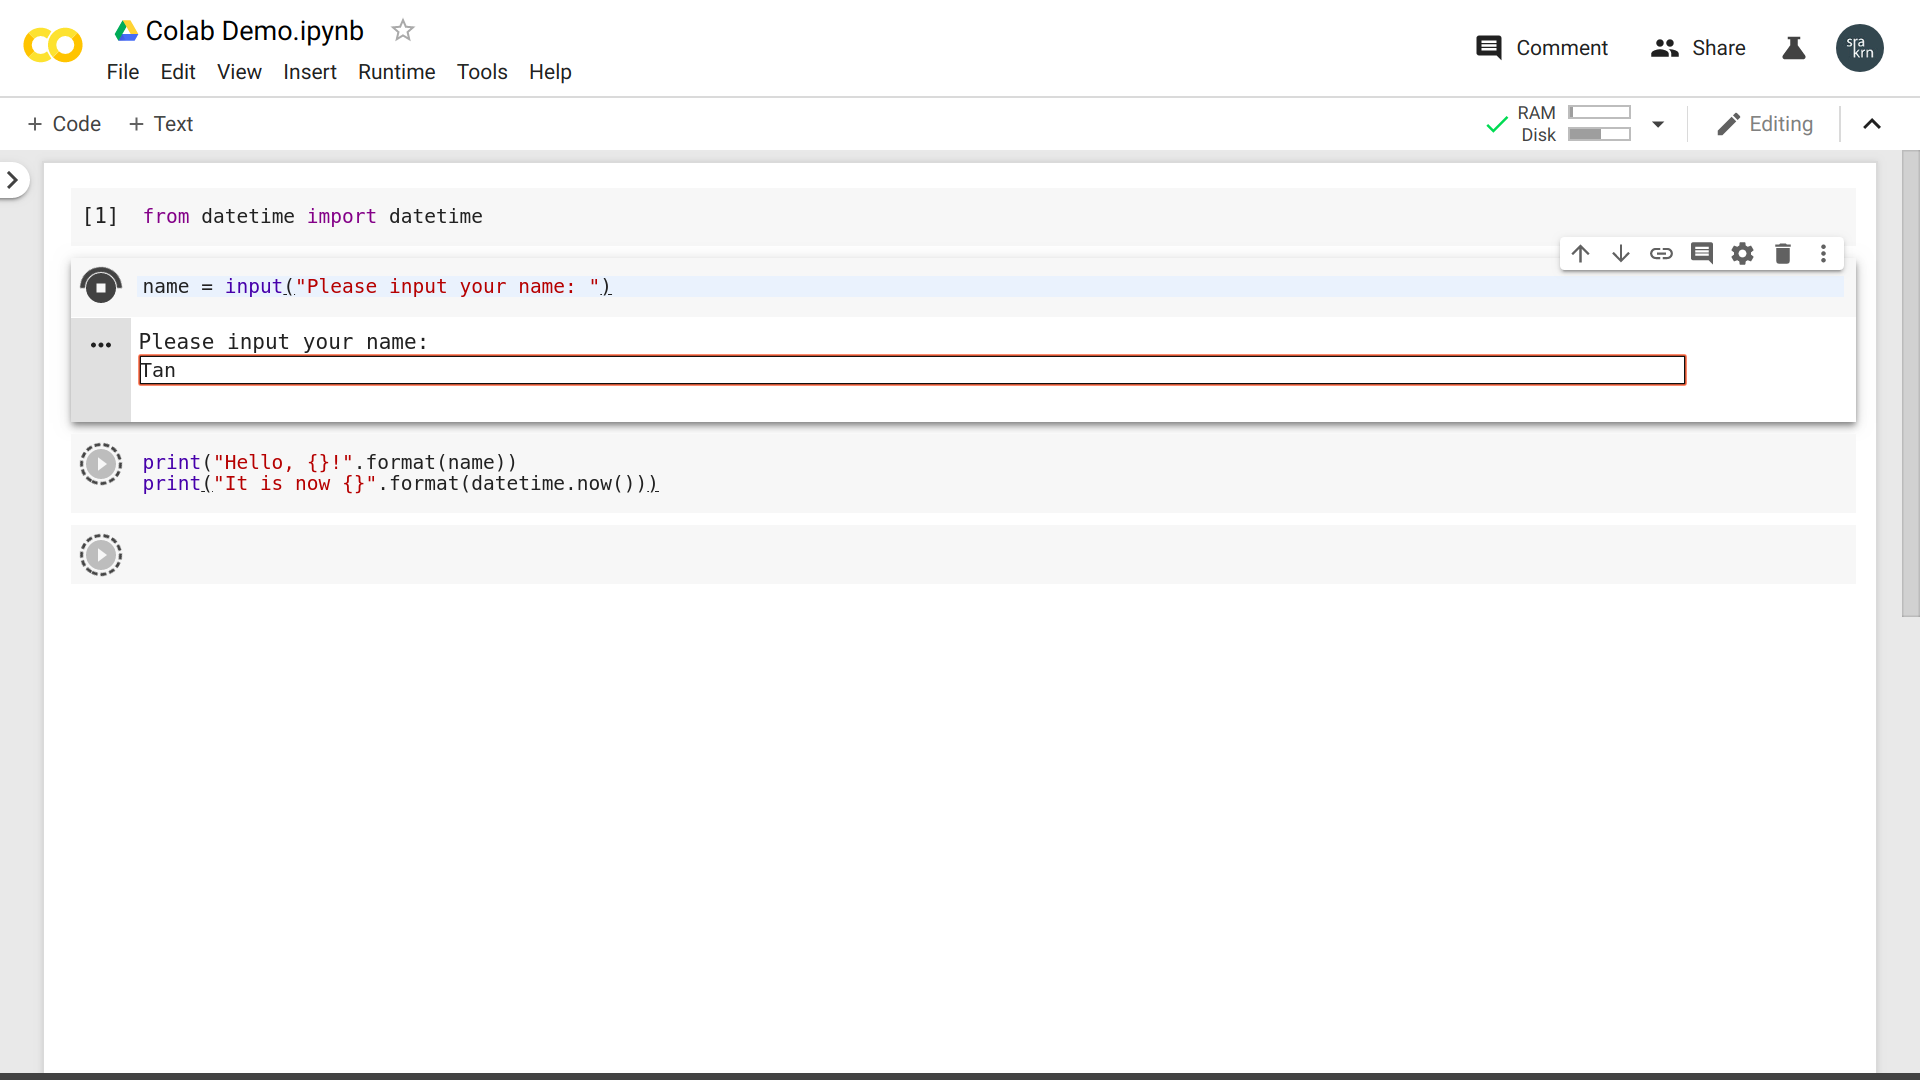
\includegraphics[width=\textwidth]{images/colab-demo.png}
\end{frame}

\begin{frame}
    \frametitle{Caveats 1: Execution order}
    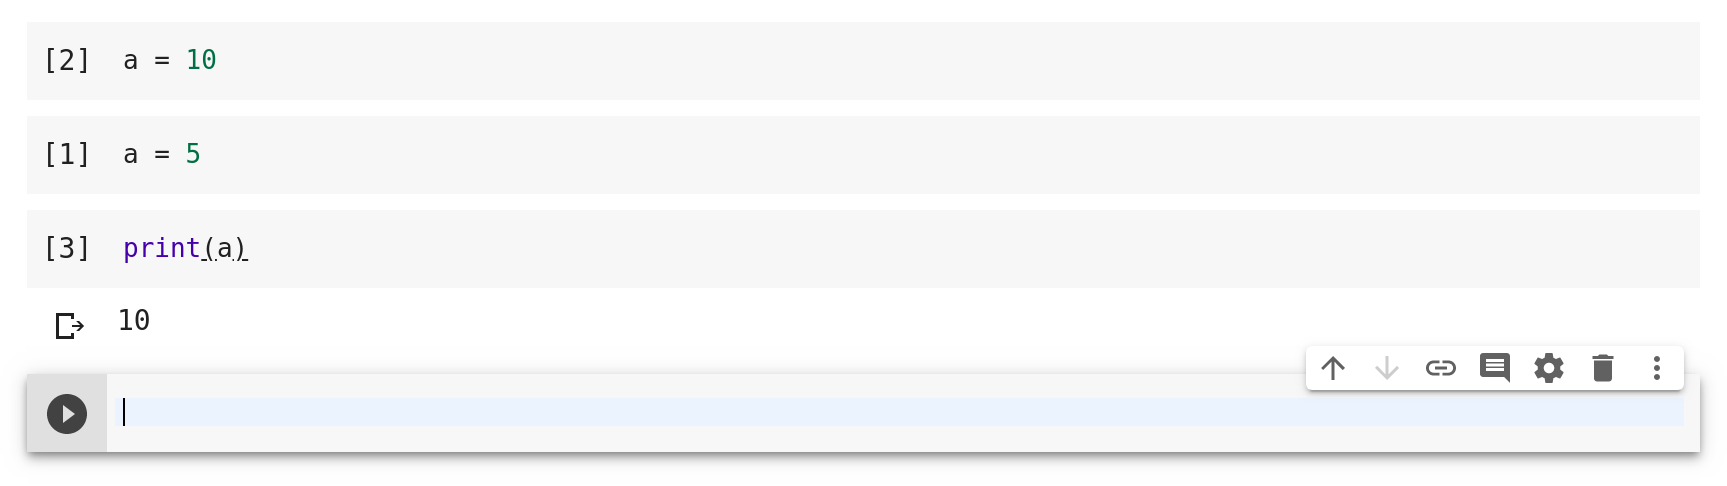
\includegraphics[width=\textwidth]{images/colab-ooo-execution.png}
    \pause
    You'll do a lot of out-of-order code execution!
\end{frame}

\begin{frame}
    \frametitle{Caveats 2: Cell edits}
    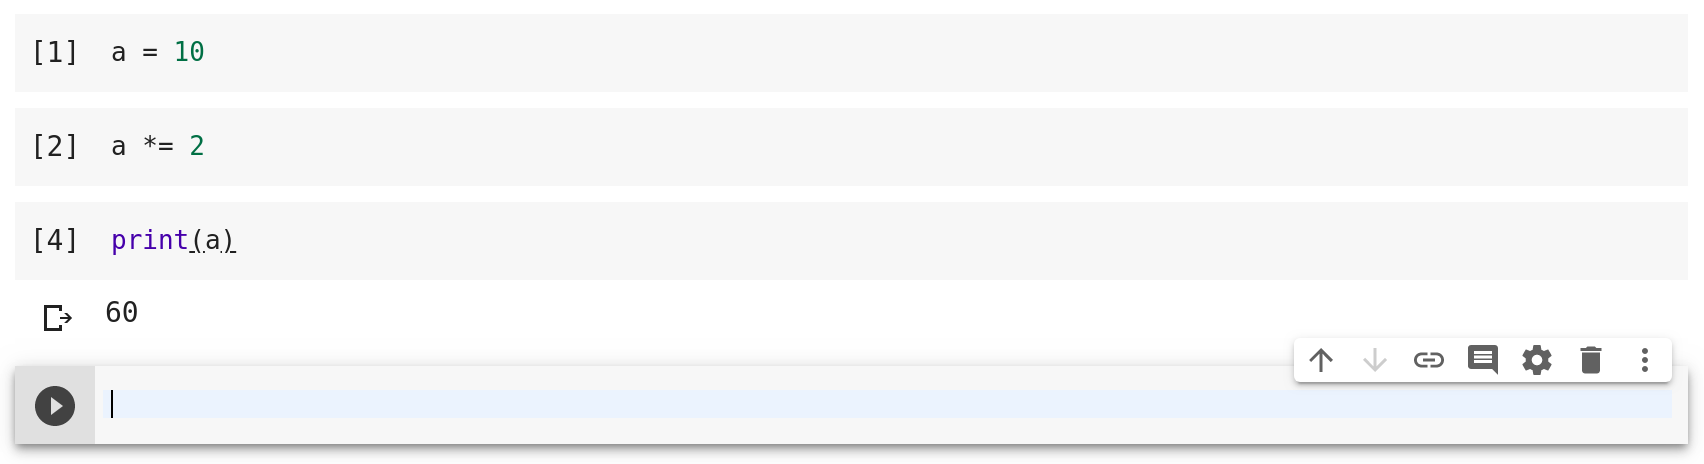
\includegraphics[width=\textwidth]{images/colab-removed-cell.png}
    \pause
    You might sometimes remove a cell, and that shows no visible trace without explicit query.
\end{frame}

\begin{frame}
    \frametitle{Caveats 2: Cell edits}
    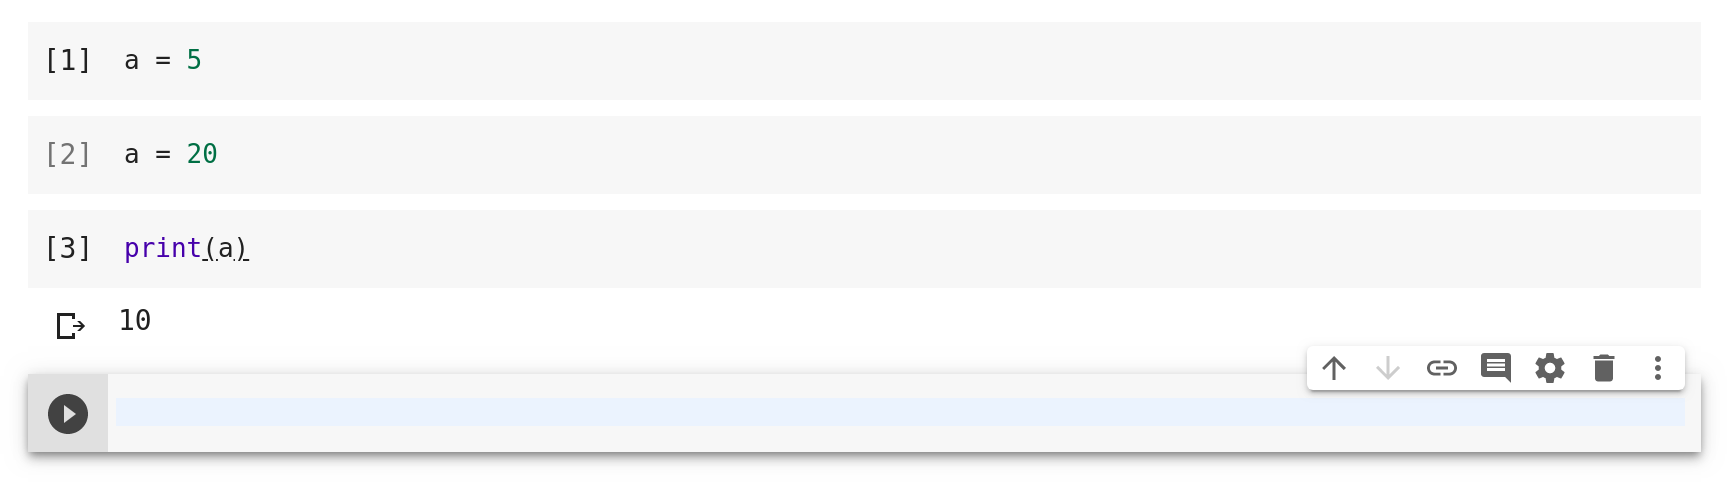
\includegraphics[width=\textwidth]{images/colab-edited-cells.png}
    \pause
    Jupyter Notebook offers no cell edited marks, while Colab offers them
    \pause
    (note: observe the greyed out cell number)
\end{frame}

\begin{frame}
    \frametitle{Caveats 3: Be neat and tidy}
    Jupyter Notebook and Colab, unlike IDE and code editors, offers a relatively poor \textbf{clean code} tools
    \begin{itemize}
        \item Syntax error highlighting
        \item Autocomplete
        \item Linting
        \item Code formatter
    \end{itemize}
\end{frame}

\begin{frame}
    \frametitle{Caveats 3: Be neat and tidy}
    \centering
    {\LARGE Sirakorn's Workflow Demo}\\
    \onslide<2-> \textit{(Please don't be amused, this is \textbf{very} normal.)}
\end{frame}

\section{Python Data Structures}

\begin{frame}[fragile]
    \frametitle{Lists}
    \begin{columns}
        \column{0.5\textwidth}
            \begin{lstlisting}[style=defaultstyle]
a = [1, 2, 3, 4, 5]
b = ["Cats", "Dogs", "Penguins", "Tonkatsu Pieces"]
c = [1, "1", True]\end{lstlisting}
        \column{0.5\textwidth}
            \begin{itemize}[<+(1)->]
                \item \textbf{Lists} are a compilation of objects.
                \item Can store multiple data types.
                \begin{itemize}
                    \item This includes storing lists in a list
                    \item So-called a \textbf{nested list}
                \end{itemize}
                \item Can be resized.
                \begin{itemize}
                    \item No need to declare its size on the first declaration.
                \end{itemize}
            \end{itemize}
    \end{columns}
\end{frame}

\begin{frame}[fragile]
    \frametitle{Lists}
    \begin{columns}
        \column{0.5\textwidth}
            \begin{lstlisting}[style=defaultstyle]
a = [1, 2, 3, 4, 5]
a[0]    # Accessing elements
a[1:3]  # Slicing
\end{lstlisting}
        \column{0.5\textwidth}
        \onslide<1-> Accessing list
            \begin{itemize}[<+(2)->]
                \item \textbf{Elementwise}: accessing one elements at a time)
                \item \textbf{Slicing}: accessing a sublist
            \end{itemize}
    \end{columns}
\end{frame}

\begin{frame}[fragile]
    \frametitle{List Functions}
    \begin{lstlisting}[style=defaultstyle]
vowels = ["a", "e", "o", "u"]

# Get a's length
len(a)
# Append the new element to the end of a
a.append("y")
# Deletes the first occurence of the element from a
a.remove("y")
# Inserts the item into a list with a specified index
a.insert(2, "i")\end{lstlisting}
\end{frame}

\begin{frame}[fragile]
    \frametitle{List Functions}
    \begin{lstlisting}[style=defaultstyle]
vowels = [1, 3, 2, 5, 4]
# Get the first index of a specified element
a.index(4)
# Sort a list and store into a new list
sorted_a = sorted(a)
# Sort a list, making changes directly to the old one
a.sort()\end{lstlisting}
\end{frame}
\end{document}